\documentclass{beamer}
\usepackage[utf8]{inputenc}
\usepackage{graphicx, epsfig}
\usepackage{amsmath,mathrsfs,amsfonts,amssymb}
%\usepackage{subfig}
\usepackage{floatflt}
\usepackage{epic,ecltree}
\usepackage{mathtext}
\usepackage{fancybox}
\usepackage{fancyhdr}
\usepackage{multirow}
\usepackage{enumerate}
\usepackage{epstopdf}
\usepackage{multicol}
\usepackage{algorithm}
\usepackage[noend]{algorithmic}
\def\algorithmicrequire{\textbf{Input:}}
\def\algorithmicensure{\textbf{Output:}}
\usetheme{default}%{Singapore}%{Warsaw}%{Warsaw}%{Darmstadt}
\usecolortheme{default}
\setbeamerfont{title}{size=\Huge}
\setbeamertemplate{footline}[page number]{}
\setbeamerfont{title}{size=\Huge}
\beamertemplatenavigationsymbolsempty

% latin bold lower
\newcommand{\ba}{\mathbf{a}} 
\newcommand{\bc}{\mathbf{c}} 
\newcommand{\be}{\mathbf{e}} 
\newcommand{\bh}{\mathbf{h}} 
\newcommand{\bp}{\mathbf{p}} 
\newcommand{\bt}{\mathbf{t}} 
\newcommand{\bu}{\mathbf{u}} 
\newcommand{\bv}{\mathbf{v}} 
\newcommand{\bw}{\mathbf{w}} 
\newcommand{\bx}{\mathbf{x}} 
\newcommand{\by}{\mathbf{y}} 
\newcommand{\bz}{\mathbf{z}} 

% latin bold upper
\newcommand{\bA}{\mathbf{A}} 
\newcommand{\bC}{\mathbf{C}} 
\newcommand{\bI}{\mathbf{I}} 
\newcommand{\bM}{\mathbf{M}} 
\newcommand{\bT}{\mathbf{T}} 
\newcommand{\bU}{\mathbf{U}} 
\newcommand{\bW}{\mathbf{W}} 
\newcommand{\bX}{\mathbf{X}} 
\newcommand{\bY}{\mathbf{Y}} 
\newcommand{\bZ}{\mathbf{Z}} 

% latin cal upper
\newcommand{\cL}{\mathcal{L}} 
\newcommand{\cN}{\mathcal{N}} 
\newcommand{\cS}{\mathcal{S}} 
\newcommand{\cT}{\mathcal{T}} 
\newcommand{\cW}{\mathcal{W}} 
\newcommand{\cX}{\mathcal{X}} 
\newcommand{\cZ}{\mathcal{Z}} 

% latin cal upper
\newcommand{\bbE}{\mathbb{E}} 
\newcommand{\bbP}{\mathbb{P}} 
\newcommand{\bbR}{\mathbb{R}} 

% greek bold lower
\newcommand{\bepsilon}{\boldsymbol{\epsilon}} 
\newcommand{\btheta}{\boldsymbol{\theta}} 
\newcommand{\blambda}{\boldsymbol{\lambda}} 
\newcommand{\bmu}{\boldsymbol{\mu}} 
\newcommand{\bsigma}{\boldsymbol{\sigma}} 
\newcommand{\bphi}{\boldsymbol{\phi}} 

% greek bold upper
\newcommand{\bSigma}{\boldsymbol{\Sigma}} 

\DeclareMathOperator*{\argmin}{arg\,min}
\DeclareMathOperator*{\argmax}{arg\,max}

\newcommand{\createdgmtitle}[1]{\title[\hbox to 56mm{Deep Generative Models  \hfill\insertframenumber\,/\,\inserttotalframenumber}]
	{\vspace{1cm} \\ Deep Generative Models \\ Lecture #1 \\ \vspace{-0.5cm}}
	\author{Roman Isachenko \\ \vspace{-0.5cm}}
	\institute{
\includegraphics[width=3cm]{../utils/ozonmasterslogo}
	\\Ozon Masters
	}
	\date{Spring, 2021}
}

\newcommand\myfootnote[1]{%
  \tikz[remember picture,overlay]
  \draw (current page.south west) +(1in + \oddsidemargin,0.5em)
  node[anchor=south west,inner sep=0pt]{\parbox{\textwidth}{%
      \rlap{\rule{10em}{0.4pt}}\raggedright\scriptsize#1}};}

\newcommand\myfootnotewithlink[2]{%
  \tikz[remember picture,overlay]
  \draw (current page.south west) +(1in + \oddsidemargin,0.5em)
  node[anchor=south west,inner sep=0pt]{\parbox{\textwidth}{%
      \rlap{\rule{10em}{0.4pt}}\raggedright\scriptsize\href{#1}{\textit{#2}}}};}
\createdgmtitle{3}
%--------------------------------------------------------------------------------
\begin{document}
%--------------------------------------------------------------------------------
\begin{frame}
%\thispagestyle{empty}
\titlepage
\end{frame}
%=======
\begin{frame}{Recap of previous lecture}
    \begin{block}{MLE problem}
    \vspace{-0.5cm}
    \[
        \btheta^* = \argmax_{\btheta} p(\bX | \btheta) = \argmax_{\btheta} \prod_{i=1}^n p(\bx_i | \btheta) = \argmax_{\btheta} \sum_{i=1}^n \log p(\bx_i | \btheta).
    \]
    \vspace{-0.5cm}
    \end{block}
    \begin{block}{Challenge}
    $p(\bx | \btheta)$ could be intractable.
    \end{block}
    \begin{block}{LVM}
    Introduce latent variable $\bz$ for each sample $\bx$
    \[
        p(\bx, \bz | \btheta) = p(\bx | \bz, \btheta) p(\bz); \quad 
        \log p(\bx, \bz | \btheta) = \log p(\bx | \bz, \btheta) + \log p(\bz).
    \]
    \[
        p(\bx | \btheta) = \int p(\bx, \bz | \btheta) d\bz = \int p(\bx | \bz, \btheta) p(\bz) d\bz.
    \]
    \end{block}
	\vspace{-0.3cm}
	\begin{block}{Motivation}
		The distributions $p(\bx | \bz, \btheta)$ and $p(\bz)$ could be quite simple.
	\end{block}
\end{frame}
%=======
\begin{frame}{Recap of previous lecture}
        \begin{block}{Incomplete likelihood maximization}
        \vspace{-0.7cm}
    	\[
    	        \btheta^* = \argmax_{\btheta} \log p(\bX| \btheta) = \argmax_{\btheta} \log \sum_{i=1}^n \int p(\bx_i| \bz_i, \btheta) p(\bz_i) d\bz_i.
    	\]
    	\vspace{-0.5cm}
	\end{block}
	\begin{block}{Variational lower bound}
		\[
		    \log p(\bx| \btheta) = \mathcal{L} (q, \btheta) + KL(q(\bz) || p(\bz|\bx, \btheta)) \geq \mathcal{L} (q, \btheta).
		\]
	\end{block}
	\begin{block}{Evidence Lower Bound (ELBO)}
	    \vspace{-0.3cm}
		\[
		    \mathcal{L} (q, \btheta) = \mathbb{E}_{q} \log p(\bx | \bz, \btheta) - KL (q(\bz) || p(\bz))
		\]
	\end{block}
	Instead of maximizing incomplete likelihood, maximize ELBO (equivalently minimize KL)
	\[
	    \max_{\btheta} p(\bx | \btheta) \quad \rightarrow \quad \max_{q, \btheta} \mathcal{L} (q, \btheta) \equiv \min_{q, \btheta} KL(q(\bz) || p(\bz|\bx, \btheta)).
	\]
	    
\end{frame}
%=======
\begin{frame}{Recap of previous lecture}
	\begin{block}{EM algorithm (block-coordinate optimization)}
	\begin{itemize}
		\item Initialize $\btheta^*$;
		\item E-step
			\vspace{-0.3cm}
			\[
				q(\bz) = \argmax_q \mathcal{L} (q, \btheta^*) = \argmin_q KL(q || p) =
				 p(\bz| \bx, \btheta^*);
			\]
			\vspace{-0.5cm}
			\begin{itemize}
				\item $p(\bz| \bx, \btheta^*)$ could be \textbf{intractable};
				\item $q(\bz)$ is different for each object $\bx$.
			\end{itemize}
		\item M-step
			\[
				\btheta^* = \argmax_{\btheta} \mathcal{L} (q, \btheta);
			\]
		\item Repeat E-step and M-step until convergence.
	\end{itemize}
	\end{block}
	\begin{block}{Amortized variational inference}
	Restrict a family of all possible distributions $q(\bz)$ to a particular parametric class $q(\bz|\bx, \bphi)$ conditioned on samples $\bx$ with parameters $\bphi$.
	\end{block}
\end{frame}
%=======
\begin{frame}{Variational EM-algorithm}

	\begin{block}{ELBO}
		\vspace{-0.1cm}
		\[
		\log p(\bx| \btheta) = \mathcal{L} (q, \btheta) + KL(q(\bz) || p(\bz|\bx, \btheta)) \geq \mathcal{L} (q, \btheta).
		\]
	\end{block}
	\begin{itemize}
		\item E-step
		\[
		\bphi_k = \bphi_{k-1} + \left.\eta \nabla_{\bphi} \mathcal{L}(\bphi, \btheta_{k-1})\right|_{\bphi=\bphi_{k-1}},
		\]
		where $\bphi$~-- parameters of variational distribution $q(\bz | \bx, \bphi)$.
		\item M-step
		\[
		\btheta_k = \btheta_{k-1} + \left.\eta \nabla_{\btheta} \mathcal{L}(\bphi_k, \btheta)\right|_{\btheta=\btheta_{k-1}},
		\]
		where $\btheta$~-- parameters of the generative distribution $p(\bx | \bz, \btheta)$.
	\end{itemize}
	Now all we have to do is to obtain two gradients $\nabla_{\bphi} \mathcal{L}(\bphi, \btheta)$, $\nabla_{\btheta} \mathcal{L}(\bphi, \btheta)$.  \\
	\begin{block}{Challenge}
		Number of samples $n$ could be huge (we heed to derive unbiased stochastic gradients).
	\end{block}
\end{frame}
%=======
\begin{frame}{ELBO gradient (M-step, $\nabla_{\btheta} \mathcal{L}(\bphi, \btheta)$)}
	\vspace{-0.3cm}
	\[
	\sum_{i=1}^n \mathcal{L}_i (\bphi, \btheta)  = \sum_{i=1}^n \mathbb{E}_{q} \left[\log p(\bx_i, \bz_i | \btheta) - \log q(\bz_i| \bx_i, \bphi) \right] \rightarrow \max_{\bphi, \btheta}.
	\]
	Optimization w.r.t. $\btheta$: \textbf{mini-batching} (1) + \textbf{Monte-Carlo} estimation (2)
	\begin{align*}
		\nabla_{\btheta} \sum_{i=1}^n \mathcal{L}_i (\bphi, \btheta)
		&= \sum_{i=1}^n \int q(\bz_i|\bx_i, \bphi) \nabla_{\btheta}\log p(\bx_i|\bz_i, \btheta)  d \bz_i \\
		&\mathrel{\stackrel{\rm (1)}\approx} n\int q(\bz_i|\bx_i, \bphi) \nabla_{\btheta}\log p(\bx_i|\bz_i, \btheta) d \bz_i , \quad i \sim U[1, n] \\
		&\mathrel{\stackrel{\rm (2)}\approx}  n \nabla_{\btheta}\log p(\bx_i|\bz^*_i, \btheta), \quad \bz^*_i \sim q(\bz_i|\bx_i, \bphi).
	\end{align*}
	\textbf{Monte-Carlo} estimation (2):
	\[
	\bbE_q f(\bz) = \int q(\bz) f(\bz) d\bz \approx f(\bz^*), \text{where } \bz^* \sim q(\bz).
	\]
\end{frame}
%=======
\begin{frame}{ELBO gradient (E-step, $\nabla_{\bphi} \mathcal{L}(\bphi, \btheta)$)}
	\vspace{-0.3cm}
	\[
	\sum_{i=1}^n \mathcal{L}_i (\bphi, \btheta)  = \sum_{i=1}^n \mathbb{E}_{q} \left[\log p(\bx_i, \bz_i | \btheta) - \log q(\bz_i| \bx_i, \bphi) \right] \rightarrow \max_{\bphi, \btheta}.
	\]
	\begin{block}{Challenge}
	Difference from M-step: density function $q(\bz| \bx, \bphi)$ depends on the parameters $\bphi$, it is impossible to use the Monte-Carlo estimation:
	\begin{align*}
		\nabla_{\bphi} \mathcal{L} (\bphi, \btheta) &= \nabla_{\bphi} \int q(\bz | \bx, \bphi) \left[\log p(\bx_i, \bz_i | \btheta) - \log q(\bz_i| \bx_i, \bphi) \right] d \bz \\
		& \neq  \int q(\bz | \bx, \bphi) \nabla_{\bphi} \left[\log p(\bx_i, \bz_i | \btheta) - \log q(\bz_i| \bx_i, \bphi) \right] d \bz \\
	\end{align*}
	\end{block}
	\vspace{-0.8cm}
	\begin{block}{Solution}
		Reparametrization trick for $q(\bz | \bx, \bphi)$ to allow the expectation is independent of parameters~$\bphi$.
	\end{block}
\end{frame}
%======
\begin{frame}{ELBO gradient (E-step, $\nabla_{\bphi} \mathcal{L}(\bphi, \btheta)$)}
	\begin{block}{Reparametrization trick}
		\vspace{-0.3cm}
		\[
		f(\xi) = \int q(\eta|\xi) h(\eta) d\eta
		\]
		Let $\eta = g(\xi, \epsilon)$, where $g$ is a deterministic function, $\epsilon$ is a random variable with a density function $r(\epsilon)$.
		{\small
		\[
			f(\xi) = \int q(\eta|\xi) h(\eta) d\eta = \int r(\epsilon) h(g(\xi, \epsilon)) d \epsilon \approx h(g(\xi, \epsilon^*)), \quad \epsilon^* \sim r(\epsilon).
		\]
		\[
			\nabla_\xi f(\xi) \approx \nabla_\xi h(g(\xi, \epsilon^*)), \quad \epsilon^* \sim r(\epsilon).
		\]}
	\end{block}
	\vspace{-0.5cm}
	\begin{block}{Example}
		\vspace{-0.5cm}
		\[
		q(\eta|\xi) = \mathcal{N}(\eta| \mu, \sigma^2), \quad r(\epsilon) = \mathcal{N}(\epsilon|0, 1), \quad \eta = \sigma \cdot \epsilon + \mu, \quad \xi = [\mu, \sigma].
		\]
	\end{block}
	\vspace{-0.5cm}
	\[
		\bepsilon \sim r(\bepsilon), \quad \bz = g(\bx, \bepsilon, \bphi), \quad \bz \sim q(\bz | \bx, \bphi).
	\]
	\begin{multline*}
		\nabla_{\bphi} \sum_{i=1}^n \mathcal{L}_i (\bphi, \btheta) =  \sum_{i=1}^n \nabla_{\bphi}\int q(\bz_i|\bx_i, \bphi) \log p(\bx_i| \bz_i, \btheta)d\bz_i  - \nabla_{\bphi} KL \\ \approx  n \nabla_{\bphi}\int r(\bepsilon) \log p(\bx_i| g(\bx_i, \bepsilon, \bphi), \btheta)d\bepsilon  - \nabla_{\bphi} KL,\quad i \sim U[1, n]   \\ \approx
		n \nabla_{\bphi} \log p(\bx_i| g(\bx_i, \bepsilon^*, \bphi), \btheta)  - \nabla_{\bphi} KL , \quad \bepsilon^* \sim r(\bepsilon).
	\end{multline*}
	
\end{frame}
%=======
\begin{frame}{ELBO gradient (E-step, $\nabla_{\bphi} \mathcal{L}(\bphi, \btheta)$)}
	\vspace{-0.3cm}
	\begin{multline*}
		\nabla_{\bphi} \sum_{i=1}^n \mathcal{L}_i (\bphi, \btheta) =  \sum_{i=1}^n \nabla_{\bphi}\int q(\bz_i|\bx_i, \bphi) \log p(\bx_i| \bz_i, \btheta)d\bz_i  - \nabla_{\bphi} KL \\ \approx  n \nabla_{\bphi}\int r(\bepsilon) \log p(\bx_i| g(\bx_i, \bepsilon, \bphi), \btheta)d\bepsilon  - \nabla_{\bphi} KL,\quad i \sim U[1, n]   \\ \approx
		n \nabla_{\bphi} \log p(\bx_i| g(\bx_i, \bepsilon^*, \bphi), \btheta)  - \nabla_{\bphi} KL , \quad \bepsilon^* \sim r(\bepsilon).
	\end{multline*}
	
	\begin{block}{Variational assumption}
		\[
		q(\bz| \bx, \bphi) = \mathcal{N} (\bmu(\bx), \bsigma(\bx)).
		\]
		\[
		\bz = g(\bx, \bepsilon, \bphi) = \bsigma(\bx) \cdot \bepsilon + \bmu(\bx).
		\]
	\end{block}
	$\nabla_{\bphi} KL (q(\bz | \bx, \bphi) || p(\bz))$ has an analytical solution.
\end{frame}
%=======
\begin{frame}{Variational autoencoder (VAE)}
	\begin{block}{Final algorithm}
		\begin{itemize}
			\item pick $i \sim U[1, n]$;
			\item compute a stochastic gradient w.r.t. $\bphi$
			\begin{multline*}
				\nabla_{\bphi} \mathcal{L} (\bphi, \btheta) = n \nabla_{\bphi} \log p(\bx_i | g(\bx_i, \bepsilon^*, \bphi), \btheta) - \\ - \nabla_{\bphi} KL (q(\bz_i|\bx_i, \bphi) || p(\bz_i)), \quad \bepsilon^* \sim r(\bepsilon);
			\end{multline*}
			\item compute a stochastic gradient w.r.t. $\btheta$
			\[
			\nabla_{\btheta} \mathcal{L} (\bphi, \btheta) = n \nabla_{\btheta} \log p(\bx_i|\bz^*_i, \btheta), \quad \bz^*_i \sim q(\bz_i|\bx_i, \bphi);
			\]
			\item update $\btheta, \bphi$ according to the selected optimization method (SGD, Adam, RMSProp).
		\end{itemize}
	\end{block}
\end{frame}
%=======
\begin{frame}{Variational autoencoder (VAE)}
	\begin{itemize}
		\item Encoder $q(\bz | \bx, \bphi) = \text{NN}_e(\bx, \bphi)$ outputs $\bmu(\bx)$ and $\bsigma(\bx)$.
		\item Decoder $p(\bx | \bz, \btheta) = \text{NN}_d(\bz, \btheta)$ outputs parameters of the sample distribution.
	\end{itemize}
	\begin{figure}[h]
		\centering
		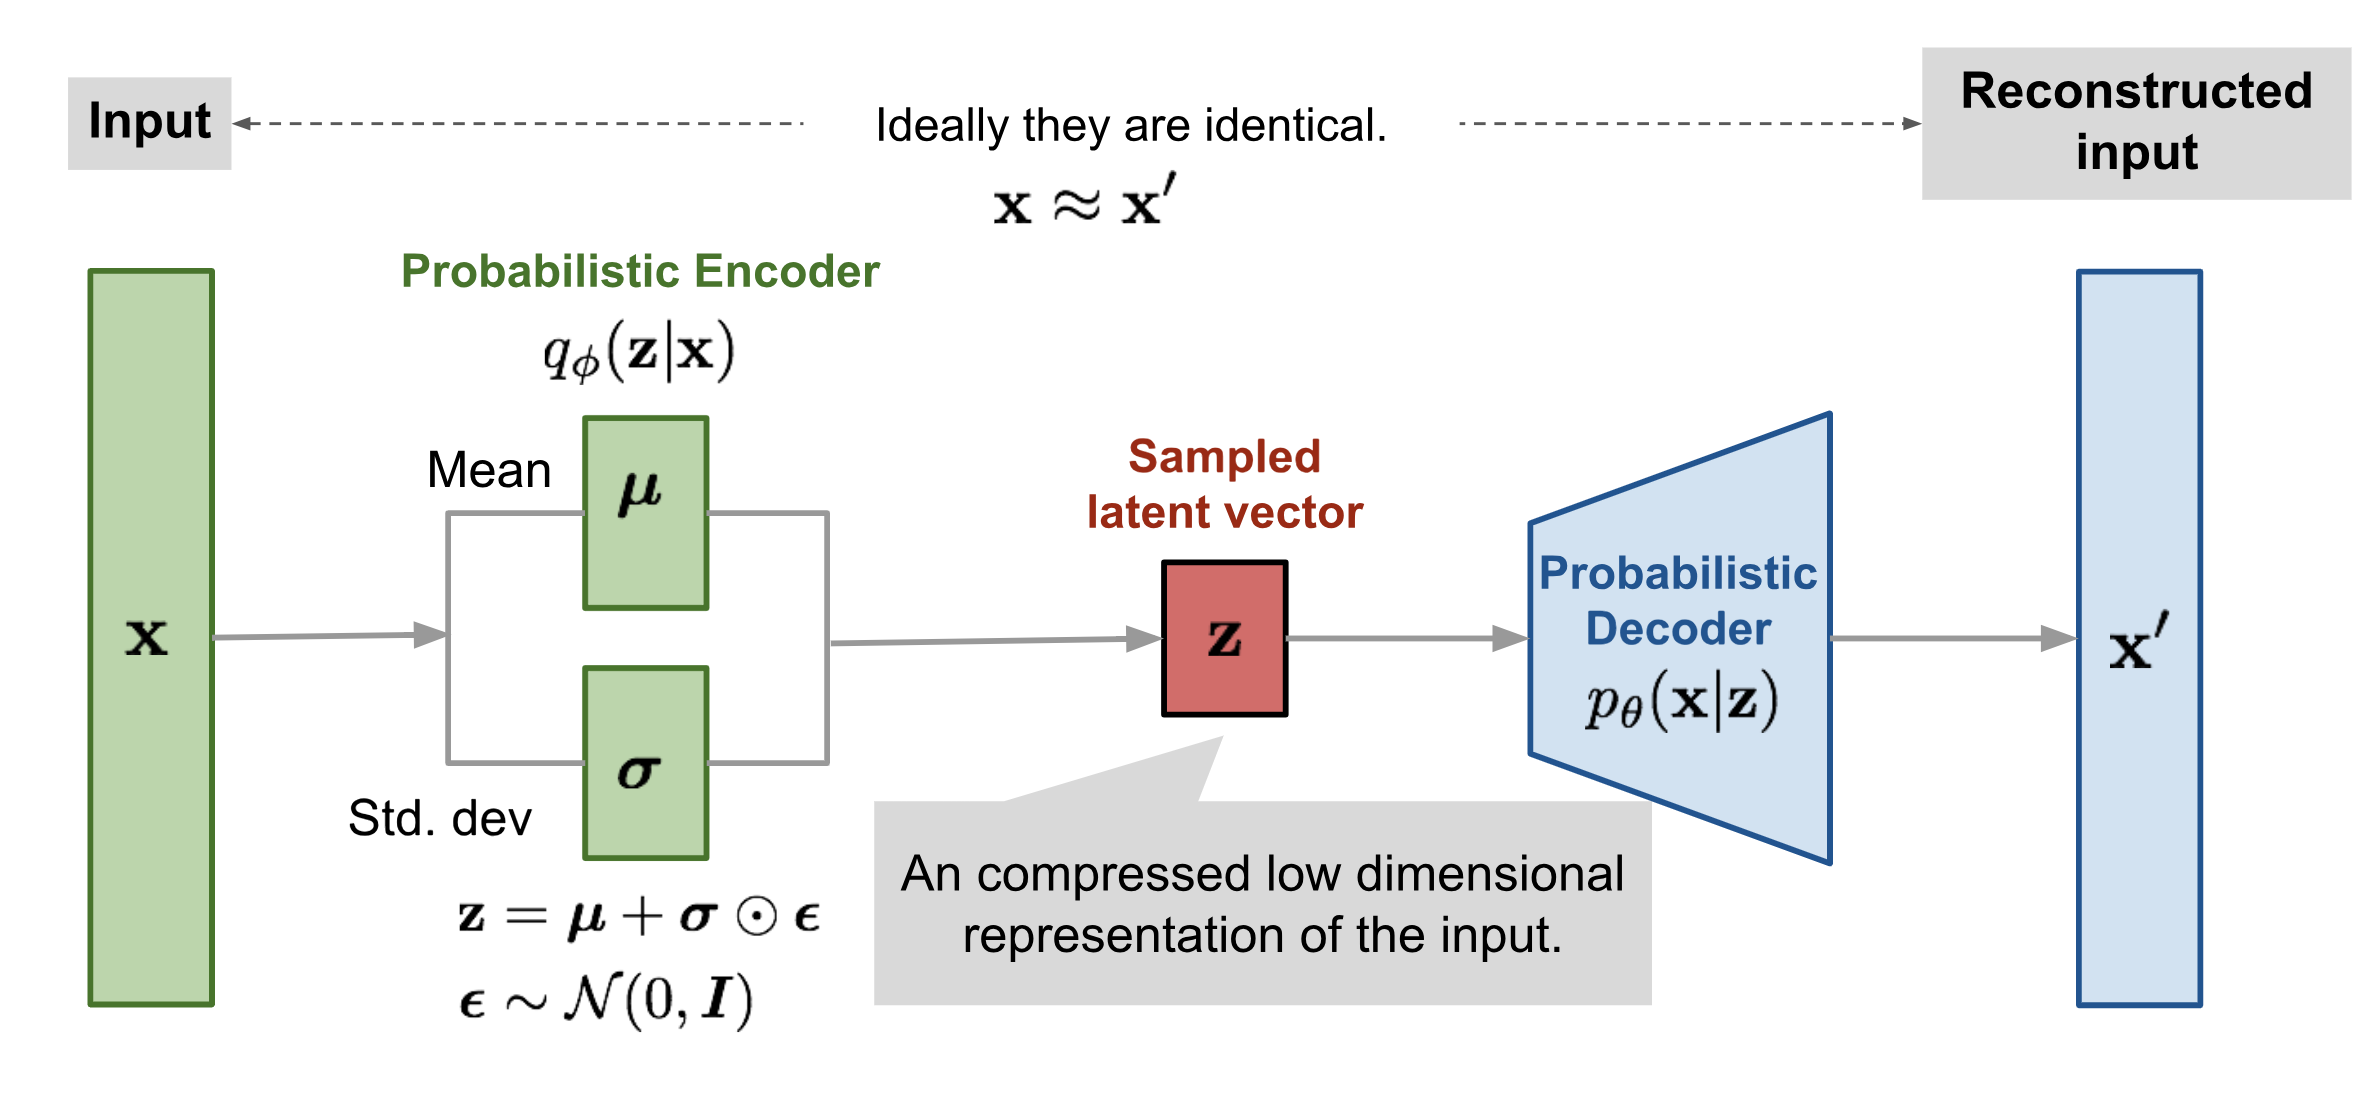
\includegraphics[width=\linewidth]{figs/vae-gaussian.png}
	\end{figure}
	
	\myfootnotewithlink{https://lilianweng.github.io/lil-log/2018/08/12/from-autoencoder-to-beta-vae.html}{image credit: https://lilianweng.github.io/lil-log/2018/08/12/from-autoencoder-to-beta-vae.html}
\end{frame}
%=======
\begin{frame}{Variational Autoencoder}
	\begin{figure}[h]
		\centering
		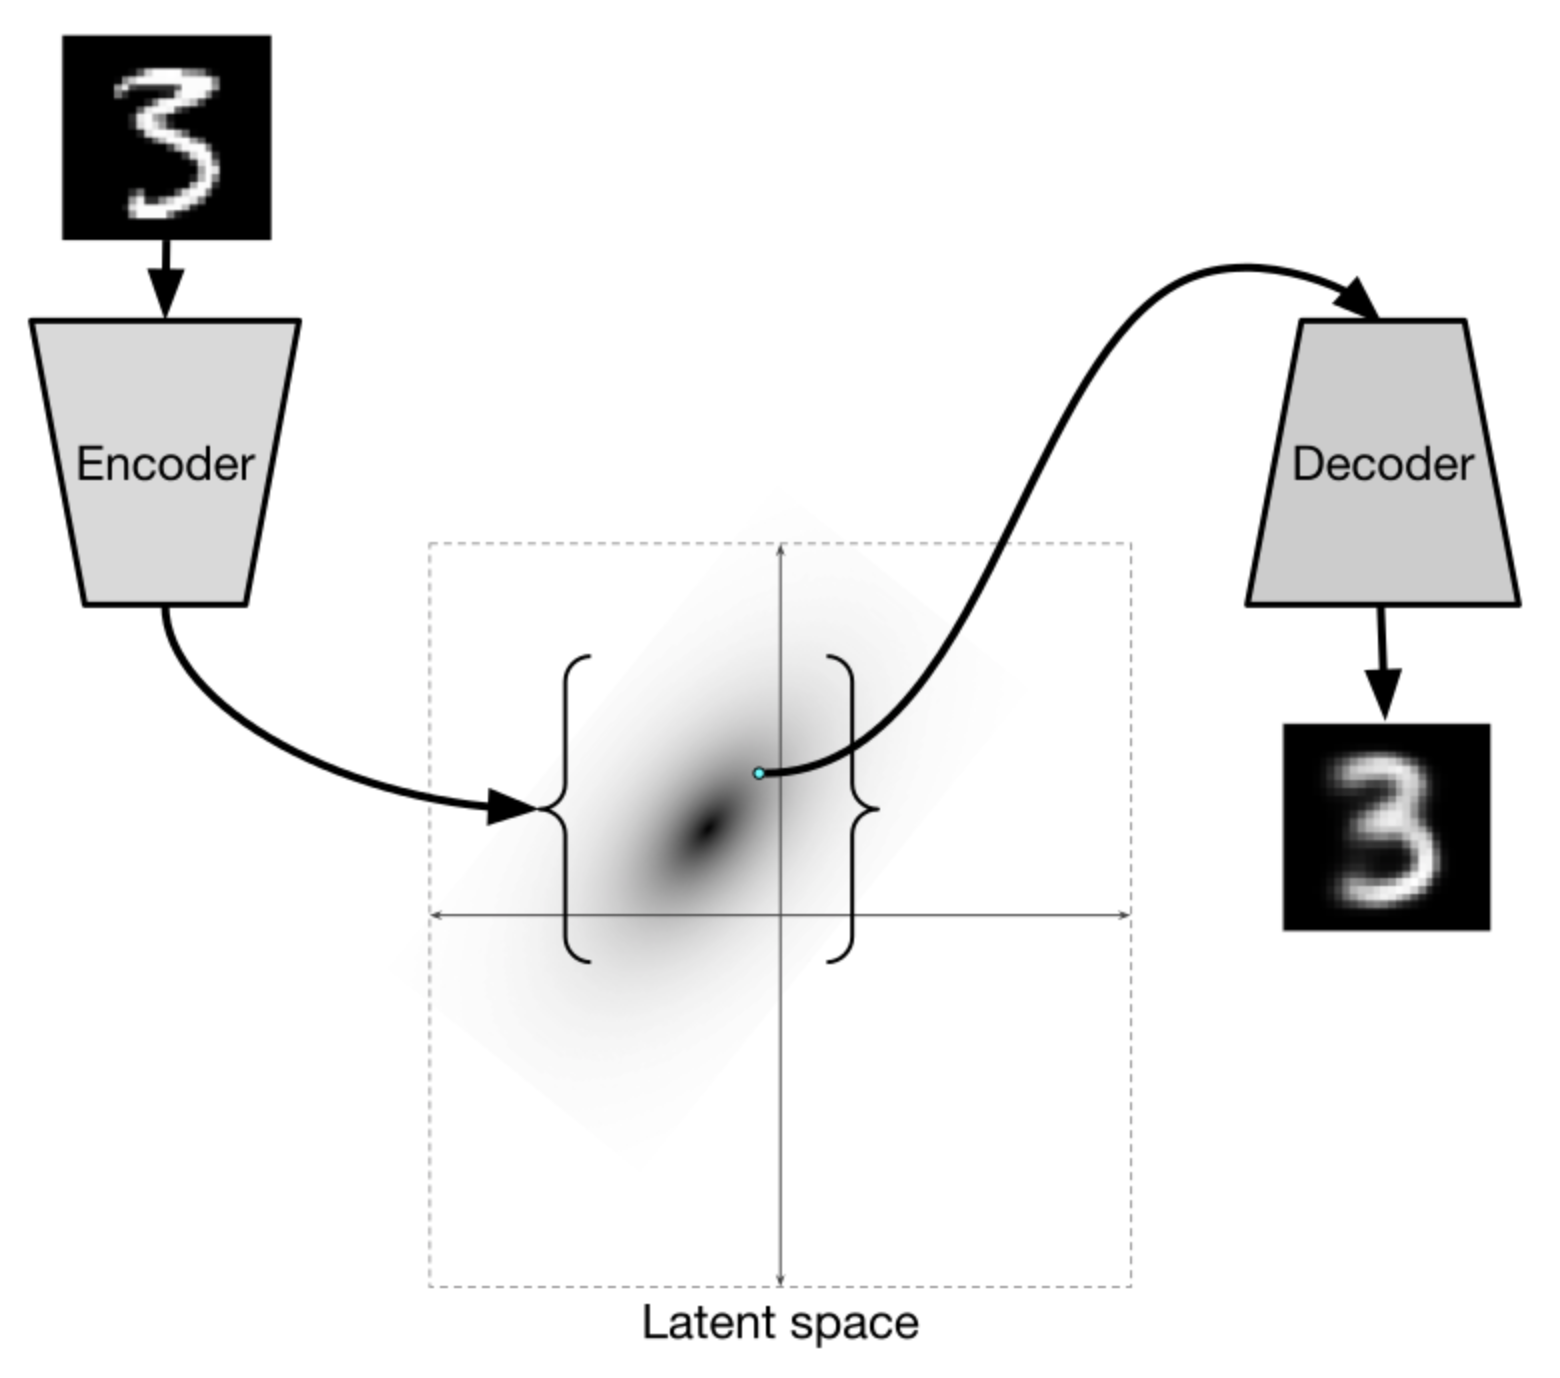
\includegraphics[width=.7\linewidth]{figs/VAE.png}
	\end{figure}
	\myfootnotewithlink{http://ijdykeman.github.io/ml/2016/12/21/cvae.html}{image credit: http://ijdykeman.github.io/ml/2016/12/21/cvae.html}
\end{frame}
%=======
\begin{frame}{Variational Autoencoder}
	Generation objects by sampling the latent space $\bz \sim \mathcal{N}(0, \mathbf{I})$
	\begin{figure}[h]
		\centering
		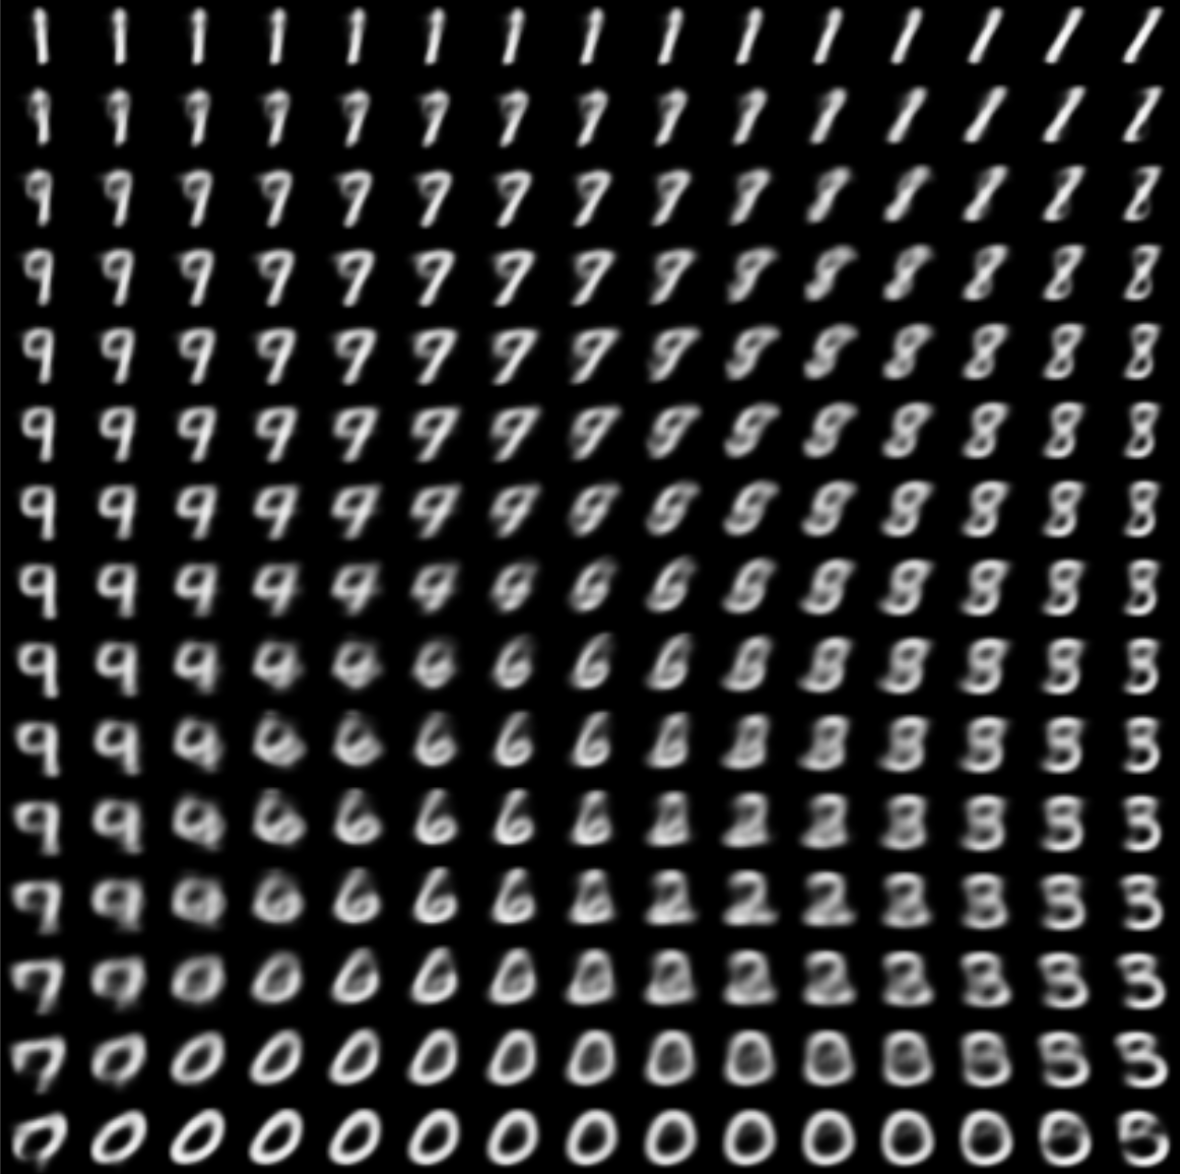
\includegraphics[width=.5\linewidth]{figs/vae_0.png}
	\end{figure}
	\myfootnotewithlink{https://habr.com/ru/post/331664}{image credit: https://habr.com/ru/post/331664}
\end{frame}
%=======
\begin{frame}{Bayesian framework}
    \begin{block}{Bayes theorem}
    \[
        p(\bt | \bx) = \frac{p(\bx | \bt) p(\bt)}{p(\bx)} = \frac{p(\bx | \bt) p(\bt)}{\int p(\bx | \bt) p(\bt) d \bt} 
    \]
    \begin{itemize}
        \item $\bx$ -- observed variables;
        \item $\bt$ -- unobserved variables (latent variables/parameters);
        \item $p(\bx | \bt)$ -- likelihood;
        \item $p(\bx)$ -- evidence;
        \item $p(\bt)$ -- prior;
        \item $p(\bt | \bx)$ -- posterior.
    \end{itemize}
    \end{block}
\end{frame}
%=======
\begin{frame}{Variational Lower Bound}
    We are given the set of objects $\bX = \{\bx_i\}_{i=1}^n$. 
    The goal is to perform bayesian inference on the latent variables $\bT = \{\bt_i\}_{i=1}^n$.
    \begin{block}{Evidence Lower Bound (ELBO)}
    \vspace{-0.3cm}
        \begin{multline*}
    		\log p(\bX) 
    		= \log \frac{p(\bX, \bT)}{p(\bT|\bX)} = \\ 
    		= \int q(\bT) \log \frac{p(\bX, \bT)}{p(\bT|\bX)}d\bT
    		= \int q(\bT) \log \frac{p(\bX, \bT) q(\bT)}{p(\bT|\bX) q(\bT)} d\bT = \\
    		= \int q(\bT) \log \frac{p(\bX, \bT)}{q(\bT)}d\bT + \int q(\bT) \log \frac{q(\bT)}{p(\bT|\bX)}d\bT = \\ 
    		= \mathcal{L} (q) + KL(q(\bT) || p(\bT|\bX)) \geq \mathcal{L} (q).
    	\end{multline*}
        \vspace{-0.3cm}
    \end{block}
	We would like to maximize lower bound $\mathcal{L}(q)$.
\end{frame}
%=======
\begin{frame}{Mean field approximation}
    \begin{block}{Independence assumption}
    \vspace{-0.3cm}
    \[
    q(\bT) = \prod_{i=1}^k q_i(\bT_i), \quad \bT = [\bT_1, \dots, \bT_k], \, \bT_j = \{ \bt_{ij}\}_{i=1}^n, \, \bt_i = \{ \bT_{ij}\}_{j=1}^k.
    \]
    \vspace{-0.3cm}
    \end{block}
    \begin{block}{Block coordinate optimization of ELBO for $q_j(\bT_j)$}
  
    {\footnotesize
    \vspace{-0.3cm}
        \begin{multline*}
    		\mathcal{L} (q)
    		= \int q(\bT) \log \frac{p(\bX, \bT)}{q(\bT)}d\bT
    		= \int \prod_{i=1}^k q_i(\bT_i) \log \frac{p(\bX, \bT)}{\prod_{i=1}^k q_i(\bT_i)}  \prod_{i=1}^k d \bT_i = \\
    		= \int \prod_{i=1}^k q_i \log p(\bX, \bT) \prod_{i=1}^k d \bT_i  
    		- \sum_{i=1}^k \int \prod_{j=1}^k q_j \log q_i \prod_{i=1}^k d \bT_i = \\
    		= \int q_j \left[\int  \log p(\bX, \bT) \prod_{i \neq j} q_i d \bT_i \right] d \bT_j - \\
    		- \int q_j \log q_j d\bT_j + \text{const}(q_j) \rightarrow \max_{q_j}
    	\end{multline*}
        \vspace{-0.3cm}}
    \end{block}
\end{frame}
%=======
\begin{frame}{Mean field approximation}
	\footnotesize
	\begin{block}{Block coordinate optimization of ELBO for $q_j(\bT_j)$}
		\vspace{-0.4cm}
	    \begin{multline*}
			\mathcal{L} (q) 
			= \int q_j \left[\int \log p(\bX, \bT) \prod_{i \neq j} q_i d \bT_i \right] d \bT_j
			- \int q_j \log q_j  d\bT_j + \text{const}(q_j) = \\
			= \int q_j \log \hat{p}(\bX, \bT_j) d \bT_j 
			- \int q_j \log q_j d\bT_j + \text{const}(q_j) \rightarrow \max_{q_j},
		\end{multline*}
		\[
		    \text{where } \log \hat{p}(\bX, \bT_j) = \mathbb{E}_{i \neq j} \log p(\bX, \bT) + \text{const}(q_j)
		\]
		\[
		    \mathbb{E}_{i \neq j} \log p(\bX, \bT) = \int \log p(\bX, \bT) \prod_{i \neq j} q_i d \bT_i.
		\]
		\vspace{-0.1cm}
		\begin{multline*}
    		\mathcal{L} (q)
    		= \int q_j (\bT_j) \log \hat{p}(\bX, \bT_j) d \bT_j - \int q_j(\bT_j) \log q_j(\bT_j) d\bT_j + \text{const}(q_j) = \\
    		 \int q_j (\bT_j) \log \frac{\hat{p}(\bX, \bT_j)}{q_j(\bT_j)} d\bT_j + \text{const}(q_j) = \\
    		= - KL (q_j(\bT_j) || \hat{p}(\bX, \bT_j)) + \text{const}(q_j) \rightarrow \max_{q_j}.
    	\end{multline*}
    \end{block}
\end{frame}
%=======    
\begin{frame}{Mean field approximation}   
	 \begin{block}{Independence assumption}
		\vspace{-0.3cm}
		\[
		q(\bT) = \prod_{i=1}^k q_i(\bT_i), \quad \bT = [\bT_1, \dots, \bT_k], \quad \bT_j = \{ \bt_{ij}\}_{i=1}^n.
		\]
		\vspace{-0.3cm}
	\end{block}
	\begin{block}{ELBO}
		\vspace{-0.3cm}
	    \[
			\mathcal{L} (q) = - KL (q_j(\bT_j) || \hat{p}(\bX, \bT_j))  + \text{const}(q_j) \rightarrow \max_{q_j}.
	    \]
	    \vspace{-0.3cm}
	\end{block}
	 \begin{block}{Solution}
	 	\vspace{-0.3cm}
		 \[
		    q_j(\bT_j) = \hat{p}(\bX, \bT_j)
		 \]
		 \[
		 	\log \hat{p}(\bX, \bT_j) = \mathbb{E}_{i \neq j} \log p(\bX, \bT) + \text{const}
		 \]
		 \[
		     \log q_j(\bT_j) = \mathbb{E}_{i \neq j} \log p(\bX, \bT) + \text{const}
		 \]
		 \vspace{-0.3cm}
	 \end{block}
\end{frame}
%=======
\begin{frame}{Mean field approximation}
	\begin{block}{ELBO}
		\[
			\mathcal{L} (q) = - KL (q_j(\bT_j) || \hat{p}(\bX, \bT_j))  + \text{const}(q_j) \rightarrow \max_{q_j}.
		\]
		\vspace{-0.3cm}
	\end{block}
	\begin{block}{Solution}
		\vspace{-0.3cm}
		\[
			\log q_j(\bT_j) = \mathbb{E}_{i \neq j} \log p(\bX, \bT) + \text{const}
		\]
		\vspace{-0.3cm}
	\end{block}
	Let assume the following factorization: $\bT = [\bT_1, \bT_2] = [\bZ, \btheta]$, and restrict the class of probability distribution for $\btheta$ to Dirac delta functions:
	\[
		q_2 = q(\bT_2) = q(\btheta) = \delta(\btheta - \btheta_0).
	\]
	
	Under the restrictions the exact solution for $q_2$ is not reached.
\end{frame}
%=======
\begin{frame}{Mean field approximation}
	\begin{block}{General solution}
		\vspace{-0.3cm}
		\[
		\log q_j(\bT_j) = \mathbb{E}_{i \neq j} \log p(\bX, \bT) + \text{const}
		\]
		\vspace{-0.3cm}
	\end{block}
	\begin{block}{Solution for $q_1 = q(\bZ)$}
		\vspace{-0.3cm}
		\begin{multline*}
			\log q(\bZ) = \int q(\btheta) \log p(\bX, \bZ,  \btheta) d\btheta + \text{const} = \\
			= \int \delta(\btheta - \btheta_0) \log p(\bX, \bZ,  \btheta) d\btheta + \text{const} = \\
			= \log p (\bZ | \bX, \btheta_0) +  \text{const}.
		\end{multline*}
	\end{block}
	\vspace{-0.3cm}
	\begin{block}{EM-algorithm (E-step)}
		\vspace{-0.3cm}
	\[
		q(\bZ) = \argmax_q \mathcal{L} (q, \btheta^*) = \argmin_q KL(q || p) = p(\bZ| \bX, \btheta^*).
	\]
	\end{block}
\end{frame}
%=======
\begin{frame}{Mean field approximation}
	\begin{block}{ELBO}
		\[
			\mathcal{L} (q) = - KL (q_j(\bT_j) || \hat{p}(\bX, \bT_j))  + \text{const}(q_j) \rightarrow \max_{q_j}.
		\]
	\vspace{-0.3cm}
	\end{block}
	\begin{block}{ELBO maximization w.r.t. $q_2 \equiv \theta_0$}
		\vspace{-0.3cm}
		\begin{align*}
			\mathcal{L} (q_2) &= - KL (q(\btheta) || \hat{p}(\bX, \btheta))  + \text{const}(\btheta_0) \\ 
			&= \int q (\btheta) \log \frac{\hat{p}(\bX, \btheta)}{q(\btheta)} d\btheta + \text{const}(\btheta_0) \\
			& = \int q (\btheta) \log \hat{p}(\bX, \btheta) d\btheta  - \int q (\btheta) \log q(\btheta) d\btheta + \text{const}(\btheta_0) \\
			& = \int \delta(\btheta - \btheta_0) \log \hat{p}(\bX, \btheta) d\btheta  - \int \delta \log \delta d\btheta + \text{const}(\btheta_0) \\ 
			& = \int \delta(\btheta - \btheta_0) \log \hat{p}(\bX, \btheta) d\btheta + \text{const}(\btheta_0) 
		\end{align*}
		\vspace{-0.3cm}
	\end{block}
\end{frame}
%=======
\begin{frame}{Mean field approximation}
	
	\begin{block}{ELBO maximization w.r.t. $q_2 \equiv \theta_0$}
		\vspace{-0.3cm}
		\[
			\mathcal{L} (q_2) = \int \delta(\btheta - \btheta_0) \log \hat{p}(\bX, \btheta) d\btheta + \text{const}(\btheta_0) = \log \hat{p}(\bX, \btheta_0).
		\]
	\end{block}
	\vspace{-0.3cm}
	\[
		\log \hat{p}(\bX, \bT_j) = \mathbb{E}_{i \neq j} \log p(\bX, \bT) + \text{const}
	\]
	\begin{align*}
		\log \hat{p}(\bX, \btheta) &= \mathbb{E}_{q_1} \log p(\bX, \bZ, \btheta) + \text{const} \\
		&= \int q(\bZ) \log p(\bX, \bZ|  \btheta) d\bZ + \log p(\btheta)+ \text{const}
	\end{align*}
	\vspace{-0.3cm}
	\begin{block}{EM-algorithm (M-step)}
		 \[
		 	\mathcal{L}(q, \btheta) =	\int q(\bZ) \log \frac{p(\bX, \bZ | \btheta)}{q(\bZ)}d\bZ \rightarrow \max_{\btheta}
		 \]
	\end{block}
\end{frame}
%=======
\begin{frame}{Mean field approximation}
    \begin{block}{Solution}
    \[
        \log q_j(\bT_j) = \mathbb{E}_{i \neq j} \log p(\bX, \bT) + \text{const}
    \]
    \end{block}

	\begin{block}{EM algorithm (special case)}
	\begin{itemize}
		\item Initialize $\btheta^*$;
		\item E-step
		\[
			q(\bZ) = \argmax_q \mathcal{L} (q, \btheta^*) = \argmin_q KL(q || p) =
			 p(\bZ| \bX, \btheta^*);
		\]
		\item M-step
		\[
			\btheta^* = \argmax_{\btheta} \mathcal{L} (q, \btheta);
		\]
		\item Repeat E-step and M-step until convergence.
	\end{itemize}
	\end{block}
\end{frame}
%=======
\begin{frame}{Summary}
\begin{itemize}
	\item Bayesian inference is a generalization of most common machine learning tasks. It allows to construct MLE, MAP and bayesian inference, to compare models complexity and many-many more cool stuff.
	\item LVM introduce latent representation of observed samples to make model more interpretable.
	\item LVM maximizes variational evidence lower bound to find MLE of model parameters.
	\item ELBO maximization is performed by the general variational EM algorithm.
	\item Amortized inference allows to efficiently compute stochastic gradients for ELBO and to use deep neural networks for $q(\bz | \bx, \bphi)$ and $p(\bx | \bz, \btheta)$.
	\item The VAE model is an LVM with an encoder network for $q(\bz | \bx, \bphi)$ and a decoder network for $p(\bx | \bz, \btheta)$.
\end{itemize}
\end{frame}
%=======
\begin{frame}{Summary}

\begin{itemize}
	\item Latent variable models introduce latent variables to the initial probabilistic model to make distribution $p(\bx | \btheta)$ tractable.
	\item To solve the MLE problem LVM optimizes the variational lower bound.
	\item The EM-algorithm is an iterative algorithm which allows to optimize the variational lower bound.
	\item VAE model is an LVM, where the encoder gives the variational distribution, the decoder defines the likelihood model.
	\item The mean field approximation is a general form of variational inference (the EM-algorithm is just a special case).
\end{itemize}
\end{frame}
%=======
\end{document} 